다음 그림에서 점 $\mathrm{I}$는 $\triangle\mathrm{ABC}$의 내심이고, 세 점 $\mathrm{D}$, $\mathrm{E}$, $\mathrm{F}$는 각각 내접원과 $\overline{\mathrm{AB}}$, $\overline{\mathrm{BC}}$, $\overline{\mathrm{CA}}$의 접점이다. $\overline{\mathrm{AB}} = 8\,\mathrm{cm}$, $\overline{\mathrm{BC}} = 10\,\mathrm{cm}$, $\overline{\mathrm{AC}} = 11\,\mathrm{cm}$일 때, $\overline{\mathrm{AF}}$의 길이는?

\begin{figure}[h]
\centering
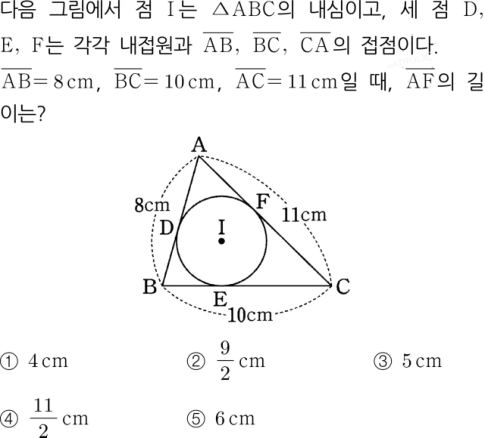
\includegraphics[width=0.4\textwidth]{plain0_problem_08_figure.png}
\end{figure}

\begin{enumerate}
    \item[①] $4\,\mathrm{cm}$
    \item[②] $\dfrac{9}{2}\,\mathrm{cm}$
    \item[③] $5\,\mathrm{cm}$
    \item[④] $\dfrac{11}{2}\,\mathrm{cm}$
    \item[⑤] $6\,\mathrm{cm}$
\end{enumerate}
